% !TEX root = sum1.tex
\section{Problem Description}

\subsection{Basic Concept}

At first, we will introduce some preliminary knowledge about our problem as follows.

We consider a set of groups to be assigned to a set of seats. For illustration, we consider the layout as $N$ rows, each row with $S_{j}$ seats, $j = 1, \ldots, N$. 

% But our model and formulation allow for a more general layout of the seats. 

The customers from the same group can sit together, while different groups should sit with social distancing. Suppose that each group has to leave one seat to maintain social distancing with the adjacent groups and different rows have no effect on each other, i.e., a person from one group can sit directly behind a person from another group.

% Considering the actual situation, the social distancing is one seat in our paper 
Let the $i-$th group type contain $i$ people. For dealing with the social distancing together, we add one to the original size of each group as the new size of the group and one dummy seat to each row. Let $s_{i} = i + 1$, $L_{j} = S_{j} +1$, $s_{i}$ is the new size of group type $i$ and $L_{j}$ is the length of row $j$.

Then the seat assignment for one row can be illustrated as below. 

\begin{figure}[ht]
    \centering
    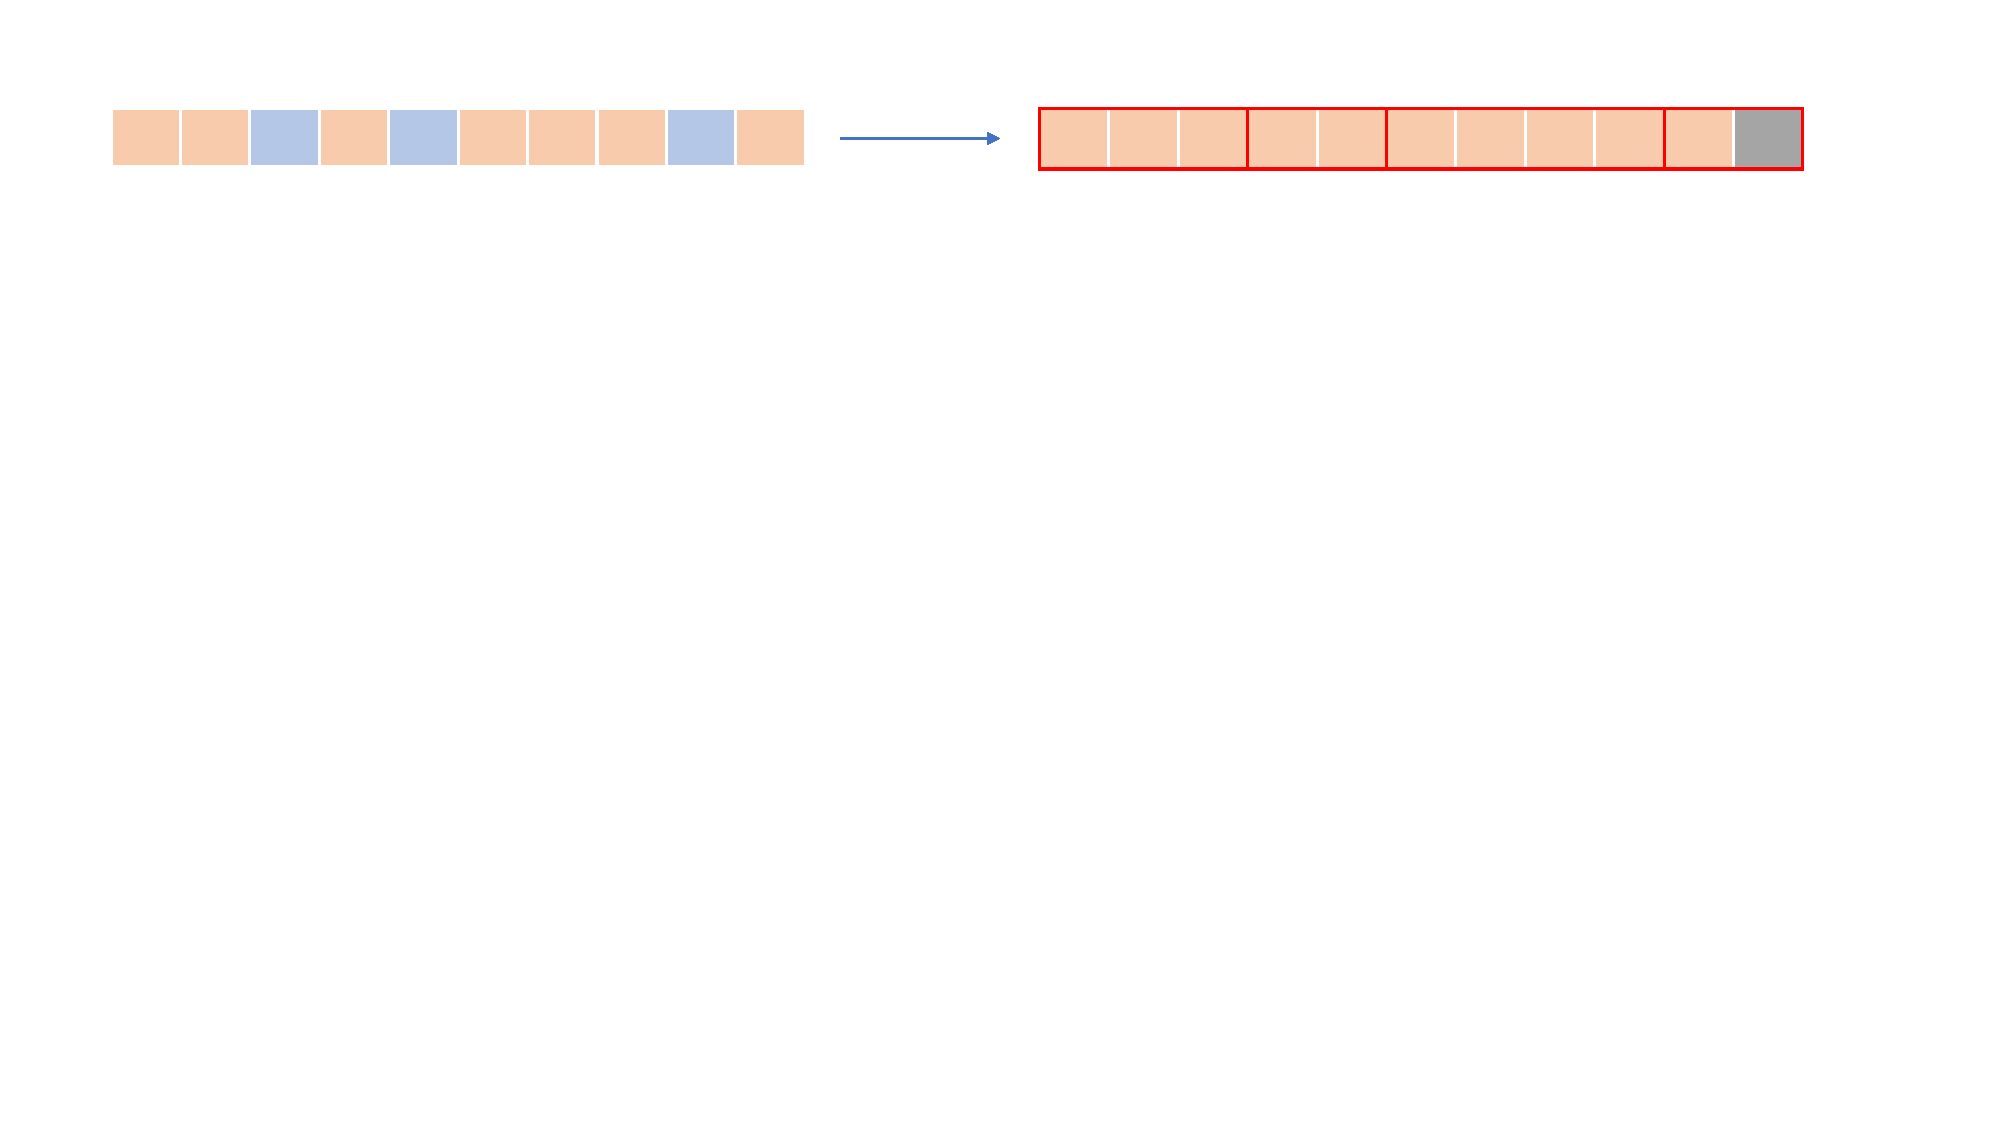
\includegraphics[width = 0.8\textwidth]{./Figures/dummy_seat.pdf}
    \caption{Problem Conversion}
\end{figure}

On the left side, the blue squares stand for the empty seats as the social distancing. The orange squares represent the seats sat by the groups. 
On the right side, one dummy seat is added at the end of the row. The orange squares surrounded by the red line are the seats taken by groups.

In this way, the social distancing will be integrated by solving this new seat assignment problem.

% The number of all seats in each row is called the length of the row.

\subsection{Deterministic Model}
We are given a demand, for example, $(d_1, d_2, d_3, d_4) = (3,5,7,6)$, where $d_i$ indicates the number of $i$-th group type.

To accommodate as many as people possible in the fixed rows, the IP formulation can be shown as below:

\begin{equation}\label{deter_upper}
    \begin{aligned}
      \max \quad & \sum_{j =1}^{N} \sum_{i = 1}^{m} (s_i -1) x_{ij} \\
      \text {s.t.} \quad & \sum_{i = 1}^{m} s_i x_{ij} \leq L_{j}, j=1,\ldots,N \\
      & \sum_{j =1}^{N} x_{ij} \leq d_{i}, i=1,\ldots,m \\
      & x_{ij} \geq 0, i=1,\ldots,m, j=1,\ldots,N.
    \end{aligned}
\end{equation}

$m$ indicates the number of group types. $x_{ij}$ indicates the number of group type $i$ placed in row $j$.

Why is it easy to solve this IP?

Because the ratio of value to capacity is monotone for the size of groups.

If the ratio is the same for the groups, IP will use more branching to obtain an optimal solution.


\subsection{Property}
Although the solver can solve this problem easily, the analyses on the property of the solution to this problem can help us generate a method for the dynamic situation. 

At first, we consider the types of pattern, which refers to the seat assignment for each row. For each pattern $k$, we use $\alpha_k, \beta_k$ to indicate the number of groups and the left seat, respectively. Denote by $l(k) = \alpha_k + \beta_k -1$ the loss for pattern $k$. The loss represents the number of people lost compared to the situation without social distancing.

Let $I_1$ be the set of patterns with the minimal loss. Then we call the patterns from $I_1$ are largest. Similarly, the patterns from $I_2$ are the second largest, so forth and so on. The patterns with zero left seat are called full patterns. We use the descending form $(t_1, t_2, \ldots, t_k)$ to represent a pattern, where $t_i$ is the new group size. 

\begin{example}\label{ex_largest}
  The length of one row is $S = 21$ and the new size of groups be $L = [2, 3, 4, 5]$. Then these patterns, $(5, 5, 5, 5, 1),(5, 4, 4, 4, 4),(5, 5, 5, 3, 3)$, belong to $I_1$. The demand is $[10, 12, 9, 8]_d$.
\end{example}

To represent a pattern with a fixed length of form, we can use a $(m+1)-$dimensional vector with $m$ group types. The aggregated form can be expressed as $[n_0, n_1, \ldots, n_m]$, where $n_i$ is the number of $i$-th group type, $i=1,\ldots,m$. 
$n_0$ is the number of left seat, its value can only be $0, 1$ because two or more left seats will be assigned to groups. Thus the pattern, $[1, 0, 0, 0, 4]$, is not full because there is one left seat.

Suppose $u$ is the size of the largest group allowed, all possible seats can be assigned are the consecutive integers from 2 to $u$, i.e., $[2,3,\ldots,u]$.
Then we can use the following greedy way to generate the largest pattern. Select the maximal group size,$u$, as many as possible and the left space is assigned to the group with the corresponding size. Let $S = u\cdot q + r$, where $q$ is the number of times $u$ selected. When $r>0$, there are $d[0][u-r][q+1]$ largest patterns with the same loss of $q$. When $r =0$, there is only one possible largest pattern.

Use dynamic programming to solve. $d[k][i][j]$ indicates the number of assignment of using $i$ capacity to allocate $j$ units, $k$ is the number of capacity allocated on the last unit. In our case, $u-r$ is the capacity need to be allocated, $q+1$ is the number of units which corresponds to the groups. Notice that we only consider the number of combinations, so we fix the allocation in ascending order, which means the allocation in current unit should be no less than the last unit.  

The number of largest patterns equals the number of different schemes that allocate $u-r$ on $q+1$ units,i.e., $d[0][u-r][q+1]$.

The recurrence relation is $d[k][i][j] = \sum_{t=k}^{i-k} d[t][i-k][j-1]$. 
When $i < k$, $d[k][i][j] =0$; when $i \geq k$, $d[k][i][1] =1$.

\begin{lem}
If all patterns associated with an integral feasible solution belong to $I_1$, then this solution is optimal.
\end{lem}

This lemma holds because we cannot find a better solution occupying more seats.

When the demand is so large that the largest patterns can be generated in all rows, an optimal seat assignment can be obtained.

\begin{prop}\label{prop_I_1}
  Let $k^{*} = \arg \max_{k\in I_1} \min_{i} \{\lfloor \frac{d_i}{b_i^k}\rfloor\}$. 
  When $N \leq \max_{k\in I_1} \min_{i} \{\lfloor \frac{d_i}{b_i^k}\rfloor\}$, the optimal seat assignment can be constructed by repeating pattern $k^*$ $N$ times.
  $N$ is the number of rows, $d_i$ is the number of $i$-th group type, $i = 1,2,\ldots, m$, $b_i^k$ is the number of group type $i$ placed in pattern $k$.
\end{prop}

Use the above example \ref{ex_largest} to explain. Take $(5,5,5,5), (5,4,4,4,4), (5,5,4,4,3)$ as the alternative patterns, denoted by pattern $1, 2, 3$ respectively. When $k = 1,2,3$. $\min_{i} \{\lfloor \frac{d_i}{b_i^k}\rfloor\}$ will be $2,3,5$, thus $k^{*}= 3$. So when $N \leq 5$, we can always select the pattern $(5,5,4,4,3)$ five times to construct the optimal seat assignment.

\begin{prop}\label{prop_I_2}
  We can construct a seat assignment in the following way. Every time we can select one pattern from $I_1$, then minus the corresponding number of group types from demand and update demand. Repeat this procedure until we cannot generate a largest pattern. If the number of generated patterns is no less than the number of rows, this assignment is optimal.
\end{prop}

% This lead

\newpage
